\documentclass[10pt,twocolumn,letterpaper]{article}

\usepackage{cvpr}
\usepackage{times}
\usepackage{epsfig}
\usepackage{graphicx}
\usepackage{amsmath}
\usepackage{amssymb}
\usepackage{breqn}
\newcommand\norm[1]{\left\lVert#1\right\rVert}
% Include other packages here, before hyperref.

% If you comment hyperref and then uncomment it, you should delete
% egpaper.aux before re-running latex.  (Or just hit 'q' on the first latex
% run, let it finish, and you should be clear).
\usepackage[breaklinks=true,bookmarks=false]{hyperref}

\cvprfinalcopy % *** Uncomment this line for the final submission

\def\cvprPaperID{****} % *** Enter the CVPR Paper ID here
\def\httilde{\mbox{\tt\raisebox{-.5ex}{\symbol{126}}}}

% Pages are numbered in submission mode, and unnumbered in camera-ready
%\ifcvprfinal\pagestyle{empty}\fi
% \setcounter{page}{4321}
\begin{document}

%%%%%%%%% TITLE
\title{Mask inpainting with a GAN network}

\author{Luca Lumetti\\
{\tt\small 244577@studenti.unimore.it}
% For a paper whose authors are all at the same institution,
% omit the following lines up until the closing ``}''.
% Additional authors and addresses can be added with ``\and'',
% just like the second author.
% To save space, use either the email address or home page, not both
\and
Federico Silvestri\\
{\tt\small 243938@studenti.unimore.it}
\and
Matteo Di Bartolomeo\\
{\tt\small 241469@studenti.unimore.it}
}

\maketitle
%\thispagestyle{empty}

%%%%%%%%% ABSTRACT
\begin{abstract}
  %% DA RIFARE UNA VOLTA FINITO TUTTO
  Our project aims to remove a face mask over a person’s face, by reconstructing
  the covered part of the face. To have a more precise reconstruction of the
  missing parts (mouth and nose) behind the mask, we plan to use a second photo
  of the same person without the mask as a reference during the facial
  reconstruction process. There are no constraints on the features of the
  reference photo, for instance the face can have a different yaw than the first
  one. To sum up the pipeline, given as input an image containing a person’s
  face partially covered by a medical mask and another photo of the same person
  without any occlusion, the output will be the first image with the
  mask-covered parts, mouth and nose, reconstructed. Future development could
  lead to generalizing the occlusion caused by the mask to any type of occlusion
  possible.
\end{abstract}

%%%%%%%%% BODY TEXT
\section{Mask Segmentation}
We made use of MediaPipe's FaceMesh \cite{DBLP:journals/corr/abs-1907-06724}
library to find facial landmarks over the face covered with the surgical mask
and the reference photo. Facial landmarks are important to have an initial
approximation of the region where to search the surgical mask and to warp the
reference photo over the first one. To perform the segmentation of the mask we
apply a k-means with k=3 over the polygon we created using specific face
landmarks and pick the bigger region between the 3.  The k has been choosen to
be 3 as in the polygonal region we expect to find the mask, the background and
the skin of the person's face. In the end, a binary image is created, with a 1
where the mask is present and 0 elsewhere, while in the original image, the mask
area is filled with 0s.
\begin{figure}
  \caption{Frontal image with landmarks on the left, resulting mask of the
  surgical mask on the right.}
  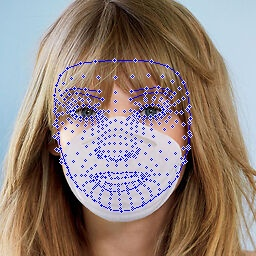
\includegraphics[width=0.49\linewidth]{img/landmarks_front.jpeg}
  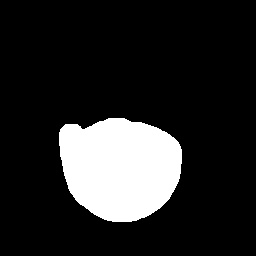
\includegraphics[width=0.49\linewidth]{img/dilated.jpeg}
\end{figure}

\section{Warping the reference photo}
The objective of the reference photo is to guide the network to a more loyal
reconstruction, by giving some informations on how the mouth and close parts
should look. As we allow the reference to have a yawn different than frontal, we
apply a thin-plate spline transformation to adjust it. We use 30 specific
landmarks as parameters as using more of them lead to distortions given by the
errors in the landmarks detection while less lead to an imperfect warping. The
same polygon region of Mask Segmentation is cut from the reference photo, the by
applying the TPS it is sticked to to main photo leading to a (partial)
reconstruction. The image will then be feeded to the network which will
reconstruct the missing parts.
\begin{figure}
  \caption{Reference photo with landmarks found by mediapipe on the left,
  resulting image on the right.}
  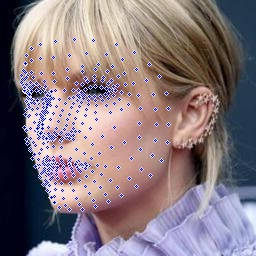
\includegraphics[width=0.49\linewidth]{img/landmarks_lateral.jpeg}
  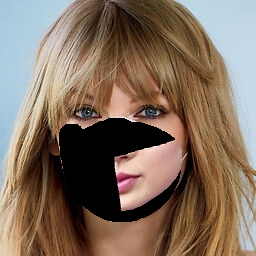
\includegraphics[width=0.49\linewidth]{img/result.jpg}
\end{figure}

\section{Image inpainting}
Image inpainting (a.k.a. image completion) is the task to fill a missing region
in an image by predicting the value of the missing pixels in order to have a
realistic image which is semantically close to the original one and visually
correct. There are two different approches to achieve this task:
\begin{enumerate}
  \item Low-level feature patch-matching which does not work pretty well with
    non-stationary use-cases (e.g. faces, objects or complicate scenes);
  \item	Feed-forward models with deep convolutional networks which overcome the
    problem of prevoious case exploiting semantics learned on large scale
    dataset.
\end{enumerate}
\section{Our approach}
We decided to follow the latter one designing a coarse-to-fine Generative
Adversarial Network (GAN) characterized by:
\begin{itemize}
	\item Generator is made of a coarse network, whose aim is to provide a rough
    estimation of the missing region, and a refinement network which takes the
    output of the previous network and the binary mask as input and improve the
    coarse output by making it more detailed.
  \item	Discriminator which is responsible of distinguishing real samples from
    the one created by the generator.
\end{itemize}
The input of the network is a pre-processed RGB image so that its values are in
range \([-1,+1]\) and its binary mask. For initializing the starting values of
the network weigths, we opted for Kaiming initialization method. We provided
different methods to initialize the starting values of the network weights, such
as normal, Xavier, orthogonal and, the default one, Kaiming.\\

We went for Adam as the generator and discriminator optimizer using a \(0.5\)
momentum and different learning rates, respectively \(0.0001\) and \(0.0004\)
for the first 10 epochs.

\subsection{Losses}
Our final loss function is given by the sum of six different losses:

\begin{dmath}
      \mathcal{L}_{tot} = \mathcal{L}_{adv} + \mathcal{L}_{recon} +
      \mathcal{L}_{tv} + \mathcal{L}_{contra} + \lambda_{perc} \cdot
      \mathcal{L}_{perc} + \lambda_{style} \cdot \mathcal{L}_{style}
\end{dmath}

Specifically, the weights $\lambda$ used are: $\lambda_{perc} = 0.05$,
$\lambda_{style} = 80$ and $\lambda_{adv} = 0.1$.\\
In the following formulas we will use symbols to refer to specific elements of
the loss function, $\mathbf{I}_{in}$ is the masked image, $\mathbf{I}_{gt}$ is
the reference ground truth image, $\mathbf{I}_{out}$ is the output of the
refinement stage, $\mathbf{I}_{com}$ is the masked image where masked pixels are
replaced with $\mathbf{I}_{out}$. \\

\subsubsection{Adversarial Loss.}
\begin{dmath}
    \mathcal{L}_{gen} = -\mathbb{E}_{\mathbf{I}_{in} \sim \mathbb{P}_i}
    [D(\mathbf{I}_{in},\mathbf{I}_{com})]
\end{dmath}
\begin{dmath}
    \mathcal{L}_{discr} = \mathbb{E}_{\mathbf{I}_{in} \sim \mathbb{P}_i}
    [\mathrm{ReLU}(1-D(\mathbf{I}_{in},\mathbf{I}_{gt}) +
    \mathrm{ReLU}(1+D(\mathbf{I}_{in},\mathbf{I}_{com})]
\end{dmath}
where \(\mathbb{P}_i\) is the data distribution of $\mathbf{I}_{in}$, \textit{D}
and \textit{G} are, respectively, the discriminator and the generator and ReLU
is the rectified linear unit defined as \(f(x) = \mathrm{max}(0,x)\).\\ It is
the GAN Hinge loss for generative adversarial learning where discriminator is
trained to distinguish $\mathbf{I}_{com}$ from $\mathbf{I}_{gt}$ and generator
has the aim of cheating the classification of the discriminator.

\subsubsection{Reconstruction Loss.}
\begin{dmath}
    \mathcal{L}_{recon} = \lambda_{hole} \mathcal{L}_{hole} +
    \mathcal{L}_{valid}
\end{dmath}
where \(\mathcal{L}_{hole}\) is the sums of the distances calculated only from
the missing pixels, \(\mathcal{L}_{valid}\) is like \(\mathcal{L}_{hole}\) but
for valid pixels. \(\lambda_{hole}\) is a weight to the pixel-wise loss withing
the missing regions.

\subsubsection{Total variation (TV) Loss.}
\begin{dmath}
    \mathcal{L}_{tv} = \sum^{H-1,W}_{x,y} \frac{\norm{ \mathbf{I}^{x+1,y}_{com}
    - \mathbf{I}^{x,y}_{com} }_1}{N^{row}_{\mathbf{I}_{com}}} +
    \sum^{H,W-1}_{x,y} \frac{\norm{ \mathbf{I}^{x,y+1}_{com} -
    \mathbf{I}^{x,y}_{com} }_1}{N^{col}_{\mathbf{I}_{com}}}
\end{dmath}
where \textit{H} and \textit{W} are the height and width of $\mathbf{I}_{com}$
and $N^{row}_{\mathbf{I}_{com}}$ and $N^{col}_{\mathbf{I}_{com}}$ are the number
of pixels in $\mathbf{I}_{com}$ without the last row and the last column.
\\
It is responsible of the regularization of the image to improve the smoothness
of the output image.

\subsubsection{Perceptual Loss.}
\begin{dmath}
    \mathcal{L}_{perceptual} = \sum^L_{l=1} \frac{\norm{
      \phi^{\mathbf{I}_{out}}_l - \phi^{\mathbf{I}_{gt}}_l
    }_1}{N_{\phi^{\mathbf{I}_{gt}}_l}} + \sum^L_{l=1} \frac{\norm{
      \phi^{\mathbf{I}_{com}}_l - \phi^{\mathbf{I}_{gt}}_l
    }_1}{N_{\phi^{\mathbf{I}_{gt}}_l}}
\end{dmath}
where \(\phi\) is the well-trained loss network, VGG-19\cite{simonyan2014very},
and \(\phi^{\mathbf{I}}_l\) the actiovation maps of the \(l^{th}\) layer of
\(\phi\) given an image \(\mathbf{I}\).
\(N_{\phi^{\mathbf{I}_{gt}}_l}\) denotes the number of elements in
\(\phi^{\mathbf{I}_{gt}}_l\) and \textit{L} is the number of layers used.
This loss represents the L1-norm distance between high-level feature
representations in 5 different convolutive layers. Its weight is set to
\(0.05\).

\subsubsection{Style Loss.}
\begin{dmath}
        \mathcal{L}_{style} = \sum^{\mathbf{I}_{out},\mathbf{I}_{com}}_{l=1}
        \sum^L_{l=1} \frac{1}{C_l C_l} \norm{ \frac{1}{C_l H_l W_l}
        ((\phi^{\mathbf{I}}_l)^\top(\phi^{\mathbf{I}}_l) -
        (\phi^{\mathbf{I}_{gt}}_l)^\top(\phi^{\mathbf{I}_{gt}}_l)  )}
\end{dmath}
where \(C_l\) refers to the number of activation maps of the \(l^{th}\) layer of
\(\phi\) and \(H_l\) and \(W_l\) are its height and width respectively. With
\((\phi^{\mathbf{I}}_l)^\top(\phi^{\mathbf{I}}_l)\) we represented the
auto-correlation matrix, the Gram matrix\cite{gatys1508neural} which computes
the features correlations between each activation map of the \(l^{th}\) layer of
\(\phi\) given the image \(\mathbf{I}\).\\
Using the same 5 levels of the previous loss, it is the sum of the distances of
the auto-correlation matrixes between the output and the ground truth multiplied
by a factor that depends on the size and number of the activation maps in those
layers. Its weigth is set to \(40\).

\subsubsection{Contrastive loss.}
\begin{dmath}\label{eq:contra}
    \mathcal{L}_{contrastive} = - \log{\frac{exp(z_{i}^\intercal
    z_{i}^{'}/\tau)}{\sum_{j=0}^{K}exp(z_{i}z_{j}^{'}/\tau)}}
\end{dmath}
The equation \eqref{eq:contra} is the categorical cross-entropy of classifying
the positive sample correctly \cite{oord2018representation}. \((z_{i},
z_{i}^{'})\) are the encoding version of the images \((x_{q}, x_{k})\), where
\(x_{q}\)is the original image and \(x_{k}\) is the trasformated image. \(\tau\)
is an hyper-parameter that control the sensitivity of the product and it's
called temperature. The dot product between the encoding vector of the original
image and the traformated image measure the similarity between rappresentations.
In our network the positive images are created by the original images with some
transformations and we don't use negative examples. This loss is helpful to get
more information during the training because the network learns from the
similarity between images. This methods try to maximise similarity between
representations of positive similar pairs and minimises the similarity with the
feature extracted from negative images\cite{le2020contrastive}.
To calculate this loss we use the feature vector with the biggest number of
channels in our network (512). We squeeze this vector in a way that preserve the
information of the original image with average pooling so we use a vector with
dimension 1x1x512. The transformations used are inspired by
StyleGAN\cite{karras2020analyzing} and they are:
\begin{itemize}
  \item horizontal flip with probability 1.0
  \item change in brightness with probability 0.75
  \item change in contrast with probability 0.75
  \item change in saturation with probability 0.75
  \item hue rotation with probability 1.0
\end{itemize}
% DA RISCRIVERE MEGLIO?
These transformations are been proven to be effective in our case as the network
was overfitting the skin color and the mouth position; some image in the FFHQ
dataset are from people with painted face (blue and red), when the network was
feeded with these images, the inpainted region wasn't of the same color of the
face. After implementing augmentation and contrastive loss, these problems
disappeared.

\subsection{Datasets}
GAN networks are data-hungry and needs a lot of diverse training examples in
order to generate quality images, for this reason we used the FFHQ 1024x1024
images \cite{karras2019style}, rescaled to 256x256.  In other GAN inpainting
architectures, the mask region to reconstruct is usually calculated during the
training in a randomized way.  As we do not need this randomization process, for
each image of FFHQ we precalculated the face region where the mask is weared
using facial landmarks. To test our network, instead, we use CelebA256 dataset
in order to compare our results with DeepGIN.

\subsection{Architecture}
Our architecture is highly inspired by Free Form Image Inpainting with Gated
Convolution \cite{yu2019free} and DeepGIN \cite{li2020deepgin}.
A mixed-precision training is used to train the network, to be more precise,
\textbf{O2} option of nvidia-apex
(https://nvidia.github.io/apex/amp.html\#o2-almost-fp16-mixed-precision) has
been used on both discriminator and generator.
Our generator net is composed of two stages: Coarse Network and Refine Network.
\begin{figure}
  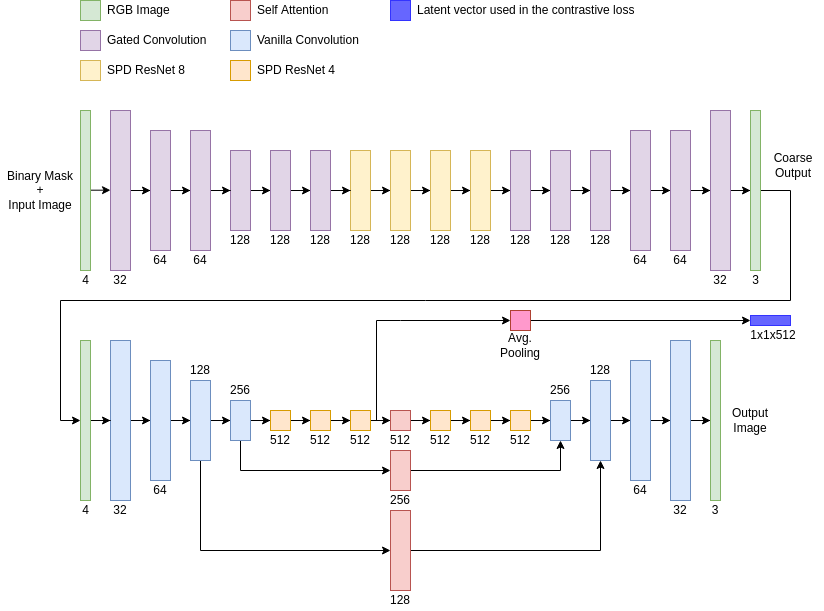
\includegraphics[width=1\linewidth]{img/generator.png}
  \caption{Generator network}
  \label{fig:generator}
\end{figure}
\begin{figure}
  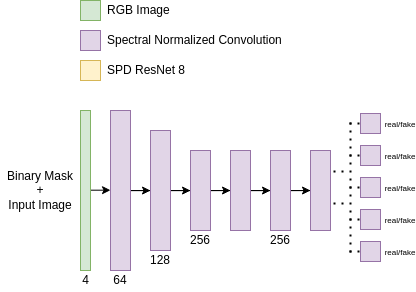
\includegraphics[width=1\linewidth]{img/discriminator.png}
  \caption{Discriminator network, GAN loss is calculated on every patch of the
  last vector}
  \label{fig:discriminator}
\end{figure}
\subsubsection{Coarse Network}
In this stage we decided to use the gated convolution so that the generator is
able to learn a dynamic feature selection mechanism for each channel and for
each spatial location. The feature selection mechanism takes into account not
only the background and the mask given in input, but also the semantic
segmentation in some channels.
Furthermore using gated convolutive layers we can avoid the inner drawbacks of
vanilla and partial convolution. In fact taking a look to the vanilla
convolution formula:
\begin{dmath}
    O_{y,x} = \sum_{i=-k'_h}^{k'_h}\sum_{j=-k'_w}^{k'_w} W_{k'_h + i, k'_w + j} \cdot I_{y + i, x + j}
\end{dmath}
where \(O_{y,x}\) is the output, \(x,y\) represent x-axis and y-axis of the
output map, \(k_h\) and \(k_w\) is the kernel size, \(k'_h = \frac{k_h -
1}{2}\),\(k'_w = \frac{k_w - 1}{2}\), \(W \in \mathbb{R}^{k_h \times k_w \times
C' \times C}\) represents the convolutional filters and \(I_{y + i, x + j}\) is
the input image, we can notice that it considers all pixels valid and it is
applied to the entire input image. This cause color discrepancy and blurriness
in final output image.
\\
In partial convolution, thanks to a masking and re-normalization step, the
operation depends only on valid pixels:
\begin{dmath}
    O_{y,x} = \begin{cases}
    \sum \sum W \cdot (I \odot \frac{M}{sum(M)}), & \text{if sum(M) \(>\) 0} \\
      0 & \text{otherwise}
    \end{cases}
\end{dmath}

\(M\) is the binary mask where a pixel with a value of 1 is considered valid and
invalid with a value of 0 and \(\odot\) is the element-wise multiplication.
There is a mask-update step based on the rule: \(m'_{y,x} = 1, \iff sum(M) > 0\)
\\
This operation, however, has some problems:
\begin{itemize}
    \item It will set to one a pixel in next layer no matter the number of
      1-value-pixels covered by the filter range in the previous layer;
    \item Invalid pixels will progressively fade out from the mask going deeper
      in the network layers;
    \item All channel in each layer shares the same mask limiting the flexibity
      of the model.
\end{itemize}
Gated convolution, instead, is based on the following formula:
\begin{gather}
    Gating_{y,x} = \sum \sum W_g \cdot I \\
    Feature_{y,x} = \sum \sum W_f \cdot I \\
    O_{y,x} = \phi (Feature_{y,x}) \odot \sigma (Gating_{y,x})
\end{gather}
where there is sigmoid function \(\sigma\) to have the output in the range
\([0,1]\), while \(\phi\) represents an activation function such ReLU, ELU and
LeakyReLU (we used the latter). \(W_g\) and \(W_f\) are two different
convolutional layers.
\\
As said before the benefits of using this operation is that the network is able
to learn a mechanism to select feature dynamically for each channel and each
spatial location considering also the semantic segmentation in some channels.
\\
As shown in figure \ref{fig:generator} the coarse net is
charaterized by an initial downsampling phase, followed by a residual one
and at the end there is and upsampling phase using the dilated gated convolution
that could be seen as a gated convolution operation preceded by a resize
operation. The output of the coarse net will pass through an activation function
(we chose a \(\tanh\)) and the result will be given as input to the refinement
network.
\subsubsection{Refine Network}
The refine network take the output of the coarse net and the mask as input.
In this stage there are 6 custom ResNet blocks with four different dilation rate and some
gated convolutional layers.
This modified ResNet blocks are called Spatial Pyramid Dilation (SPD) (Figure
\ref{fig:rnspd}). This layer is composed of different convolutional blocks with
different dilation, and the output of these blocks is concatenated together.
With different value of dilation rate we can take information from a bigger
receptive field.
\begin{figure}
  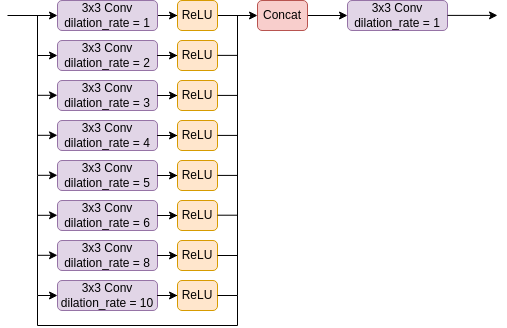
\includegraphics[width=1\linewidth]{img/SPDresnet.png}
  \caption{ResNetSPD block with 8 different dilation rate used in the coarse
  network}
  \label{fig:rnspd}
\end{figure}
Another useful feature that is implemented in this net is the Multi Scale Self
Attention (MSSA). The MSSA using the self-similarity between different layers
and it's helpful to have a better coherence in the final image. We control
the self-similarity with three different scale: 16x16, 32x32, 64x64.
The central layer are composed of self attention block. We use standard
convolutional layer to reduce the size before the self attention. In this manner
we avoid an excessive increase of the parameters. With self attention we can
find a better correlation between feature and we have a better reconstruction.
\subsubsection{Discriminator}
Our discriminator is composed by 6 convolutional blocks with kernel size 5 and
stride 2.
These convolutional methods allow to captures the Markovian patches that
represents better contextual feature\cite{li2016precomputed}.
We add a spectral normalization to improve the training
stabilization\cite{miyato2018spectral}.
The input of this network is the image (real or fake) and the relative mask.
\begin{dmath}
        \mathcal{L}_{D^{sn}}= \mathbb{E}_{x\sim \mathbb{P}_{data(x)}} \left [
          ReLU(1-D^{sn}(x))) \right ] + \mathbb{E}_{z\sim \mathbb{P}_{data(x)}}
        \left [ ReLU(1+D^{sn}(G(z)))\right ]
\end{dmath}

where \(D^{sn}\) is the spectral-normalized discriminator and G is the generator
that create the image z.

\subsection{Multi-GPU and Multi-Node Training}
% Da rivedere
As GAN networks are heavy to train, we decided to design the whole network to be
trainable on multi GPU and multi node architectures. Training it on a single K80
was infeasible as a batch size greater that 2 gives CUDA out of memory error.
We end up using 4 GPU K80 in parallel that let us to complete a full epoch in
under 24h (which is the time limit on AImageLab's servers). We also give support
for multi node because even if we were on the same node, we initially could use
at most 2 GPUs per account, so every account could be seen as a different node
thus we could break the GPUs limit. Anyway as our max GPU per users were
upgraded to 4, we didn't use that technique.

\subsection{Results}
To evaluate the results (Table \ref{tab:results}) we use different metrics:
PSNR, SSIM, LPIPS and FID. We conducted the test with CelebA 256 Dataset and
compared the results with different inpainting network. It must be noted that
our network is the only one who is restricted to inpaint a specific part of an
image of a human face, others generalize
There are no network out there which perform our same specific tasks.
\begin{table}
  \begin{tabular}{|c|c|c|c|c|c|}
    \hline
    Method & PSNR & SSIM & FID & LPIPS \\
    \hline
    DeepFillv2 (FFHQ) & 29.70 & 0.72 & 75.56 & 0.29 \\
    DIP (CelebA)      & 25.46 & 0.85 & n.d. & n.d. \\
    Ours (CelebA)     & 58.95 & 0.88 & 151.95 & 0.23\\
  \hline
  \end{tabular}
  \\
  \caption{Comparison with different network on the same metrics}
  \label{tab:results}
\end{table}

Results are not that bad, FID is pretty high and we think that this is due to
some artifacts that often appears in the generated regions.
In the Table \ref{tab:photos} we show some of the generated images.
\begin{table}
  \begin{tabular}{cccc}
    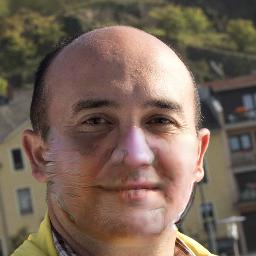
\includegraphics[width=.24\linewidth]{samples/00045.jpg}&
    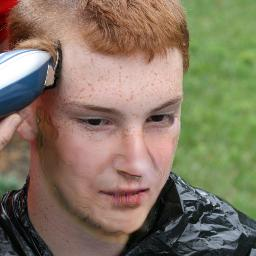
\includegraphics[width=.24\linewidth]{samples/00053.jpg}&
    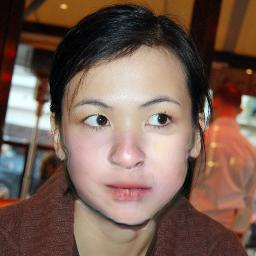
\includegraphics[width=.24\linewidth]{samples/00099.jpg}&
    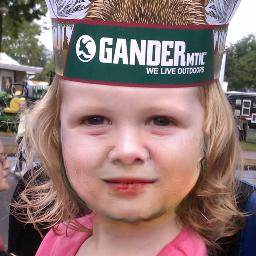
\includegraphics[width=.24\linewidth]{samples/00146.jpg}\\
    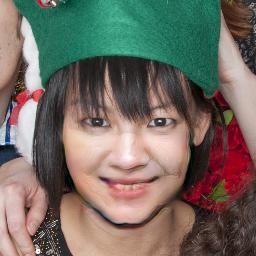
\includegraphics[width=.24\linewidth]{samples/00202.jpg}&
    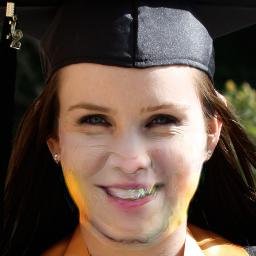
\includegraphics[width=.24\linewidth]{samples/00298.jpg}&
    
\includegraphics[width=.24\linewidth]{samples/00353.jpg}&
    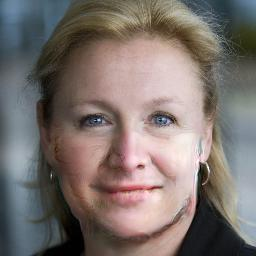
\includegraphics[width=.24\linewidth]{samples/00708.jpg}\\
    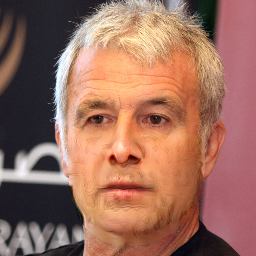
\includegraphics[width=.24\linewidth]{samples/recon_600.png}&
    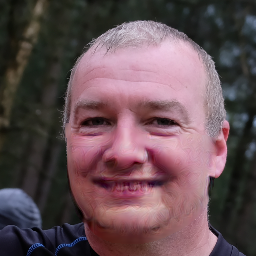
\includegraphics[width=.24\linewidth]{samples/recon_900.png}&
    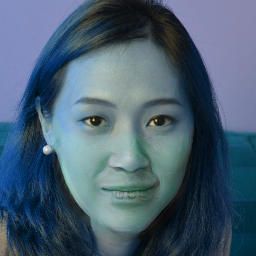
\includegraphics[width=.24\linewidth]{samples/aug_recon_1600.png}&
    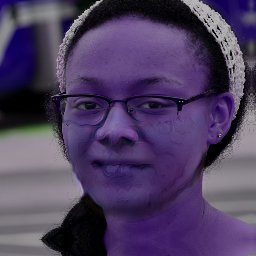
\includegraphics[width=.24\linewidth]{samples/aug_recon_200.png}\\
\end{tabular}
  \label{tab:photos}
  \caption{Some of the generated images, the latter two were augmented before
  feeding them to the network.}
\end{table}

\subsection{Conclusion}
Our results are not too far to the state-of-the-art and we think that they can be
improved by training the network for more time and more data. Some of the
networks we have compared had \~10x more epochs and used a lot more training data (CelebA + FFHQ + StyleGAN).
We couldn't afford that as the time and computing resource were not feasible for
us.\\ This network is also differ from the other because it has a specific inpainting
tasks, while the other networks have to generalize to a larger domain.

%% ALTRO?

{\small
\bibliographystyle{plain}
\bibliography{cvproject}
}

\end{document}
